% !TEX root = ./Vorlesungsmitschrift DIFF 2.tex  
\lecture{Mo 08.06. 10:15}{}
\section{Tangential- und Normalraum}
\begin{erinnerung*}
  \( \tangentialraum{M}=\Kern-{Df(a)} \), wo \( f \) eine lokale Beschreibung von \( M \) bei \( a \) als Nullstellengebilde ist.

  \begin{equation*}
    \tangentialraum{M}=\Bild{D\varphi(x_0)}=\Span-{\Set{\begin{pNiceMatrix} 1 \\ 0 \\ \Vdots \\ 0 \\ \partial_1 g(x_0) \end{pNiceMatrix},\dotsc,\begin{pNiceMatrix} 0 \\ 0 \\ \Vdots \\ 1 \\ \partial_d g(x_0) \end{pNiceMatrix}}},
  \end{equation*} 
  wo \( \varphi(x)=(x,g(x)) \) die zu einer lokalen Beschreibung von \( M \) bei \( a \) als Graph gehörige Graphenabbildung ist und \( a=(x_0,g(x_0)) \).
\end{erinnerung*}
Es gilt allgemeiner
\begin{satz}\label{tangentialraum_durch_parametisierung}
  Sei \( M \) \( d \)-dimensionale Untermannigfaltigkeit des \( \reals^n \). Sei \( a\in M \), \( U\subset \reals^n  \) offene Umgebung von \( a\) und \( \varphi\maps V\to M\cap U \) eine lokale Parametrisierung von \( M \) bei \( a \), also \( \varphi\maps V\to \reals^n \), \( V\subset \reals^d \) offen, ist \( \stetigefunktionen[1]\), \( D\varphi(t) \) von maximalem Rang \( d \) für alle \( t\in V \), \( \varphi\maps V\to M\cap U \) Homöomorphismus. Sei \( t_0\in V \) \sd \( \varphi(t_0)=a \). Dann ist \( \tangentialraum{M}=\Bild-{D\varphi(t_0)} \), also
  \begin{equation}
    \tangentialraum{M}=\Span-{\set{\braceannotate{\text{Basis von \( \tangentialraum{M} \)}}{\partial_1\varphi(t_0),\dotsc,\partial_d \varphi(t_0)}}}.
  \end{equation}
\end{satz}
\begin{proof}
  \begin{equation*}
    \rang-{D\varphi(t_0)=d\implies \dim-{\Bild-{D\varphi(t_0)}}}=d\quad \checkmark.
  \end{equation*}
  \begin{proofdescription}
    \item[\( \tangentialraum{M}\subset \Bild-{D\varphi(t_0)} \)]
    Sei \( v=v_1\partial_1 \varphi(t_0)+\dotsb+v_d\partial_d \varphi(t_0) \), \( v_j\in \reals \). Betrachte 
    \begin{gather*}
      \gamma\maps \ointerval{-\varepsilon}{\varepsilon}\to M\cap U\\
      \gamma(s)\definedas \varphi(t_0+s\underline{v})
    \end{gather*}
    mit \( \underline{v}=\transpose-{(v_1,\dotsc,v_d)}\in \reals^n \) und mit \( \varepsilon \) so klein gewählt, dass \( t_0+s\underline{v}\in V \) für alle \( s\in \ointerval{-\varepsilon}{\varepsilon} \). Dann gilt: \( \gamma(0)=\varphi(t_0)=a \) und \( \gamma \) ist stetig differenzierbar und
    \begin{align*}
      \gamma'(0)&=D\varphi(t_0)\matrixmult \underline{v}\\
      &=\partial_1 \varphi(t_0)\cdot v_1+\dotsb+\partial_d\varphi(t_0)\matrixmult v_d\\
      &=v.
    \end{align*}
    \item[\( \tangentialraum{M}\supset \Bild-{D\varphi(t_0)} \)] Sei also \( v\in \tangentialraum{M} \), \( \gamma\maps \ointerval{-\varepsilon}{\varepsilon}\to M\cap U \) stetig differenzierbar mit \( \gamma(0)=a \), \( \gamma'(0)=v \). Dann ist \( c=\inverse{\varphi}\circ \gamma\maps \ointerval{-\varepsilon}{\varepsilon}\to V  \) stetig differenzierbar (das folgt wie im Beweis von \( \ref{parameterwechsel} \) aus der Verknüpfung mit einem Diffeomorphismus \( F\maps \tilde{U}\to W \) mit
    \begin{equation*}
      F(M\cap \tilde{U})=\set{a\in W|y_j=0\quad j\geq d+1}.
    \end{equation*} 
    \Obda \( U=\tilde{U} \), somit ist
    \begin{equation*}
      \inverse{\varphi}\circ \gamma=\inverse{(\braceannotate{=(f,0)\text{\ Diffeo}}{F\circ \varphi})}\circ (F\circ \gamma)
    \end{equation*}
    \( \stetigefunktionen[1] \).) Es gilt (Kettenregel!)
    \begin{align*}
      v&=\gamma'(0)\\
      &=(\varphi\circ c)'(0)\\
      &=D\varphi(\braceannotate{=\inverse{\varphi}(a)=t_0}{c(0)}\matrixmult c'(0))\\
      &=\partial_1 \varphi(t_0)\matrixmult\braceannotate{\in \reals}{c_1'(0)}+\dotsb+\partial_d \varphi(t_0)\matrixmult\braceannotate{\in \reals}{c_d'(0)},
    \end{align*}
    also \( v\in \Span-{\set{\partial_1 \varphi(t_0),\dotsc,\partial_d\varphi(t_0)}} \).
  \end{proofdescription}
  \begin{figure}[H]
    \centering
    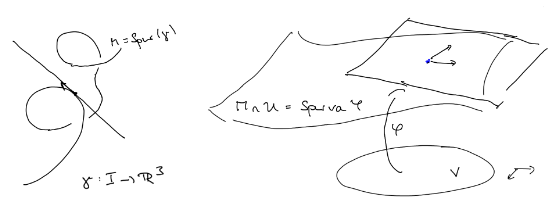
\includegraphics[width=0.5\linewidth]{tangentialraum_durch_parametisierung}
    \caption*{\( T_{\gamma(t)}M=\Set{\lambda\gamma'(t)|\lambda\in \reals} \).}
    \label{fig:tangentialraum_durch_parametisierung}
  \end{figure}
\end{proof}
\begin{beispiel*}
  \( \sphere{2}\subset \reals^2 \), \( a=\transpose-{(0,0,1)} \).
  \begin{eigenschaftenenumerate}
    \item
    \begin{align*}
      f(x)&=1-x_1^2-x_2^2-x_3^2\\
      Df(x)&=-2(x_1,x_2,x_3)\\
      \tangentialraum{M}&=\Kern-{D(a)}=\Kern{-2\transpose-{e_3}}\\
      &=\perpspace-{\Set{e_3}}=\Span-{\set{e_1,e_2}}.
    \end{align*}
    \item \( \varphi\maps D=\Set{x\in \reals^2|\euclidiannorm{x}<1} \to \reals^3\), \( \varphi(x)=\transpose-{(x,\sqrt{1-x_1^2-x_2^2})} \),
    \begin{align*}
      \partial_1 \varphi(x)&=\begin{pNiceMatrix} 1 \\ 0 \\ \frac{-x_1}{\sqrt{\cdots}} \end{pNiceMatrix}\\
      \partial_2 \varphi(x)&=\begin{pNiceMatrix} 0 \\ 1 \\ \frac{-x_2}{\sqrt{\cdots}} \end{pNiceMatrix}\\
      a&= \varphi(0)\\
      \implies \tangentialraum{M}&=\Span-{\Set{\begin{pNiceMatrix} 1 \\ 0 \\ 0 \end{pNiceMatrix},\begin{pNiceMatrix} 0 \\ 1 \\ 0 \end{pNiceMatrix}}}.
    \end{align*}
    \item \( \varphi\maps \ointerval{0}{\pi}\times\ointerval{0}{2\pi} \to \reals^3\), \( \varphi(\beta,\alpha)=\transpose-{(\Cos{\beta},\Cos{\alpha}\Sin{\beta},\Sin{\alpha}\Sin{\beta})} \). \approxtimestamp{15}
    \begin{figure}[H]
      \centering
      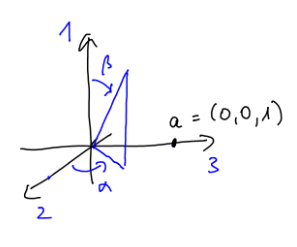
\includegraphics[width=0.5\linewidth]{winkelparametisierung_kugel}
      \label{fig:winkelparametisierung_kugel}
    \end{figure}
    \begin{align*}
      \partial_1\varphi(\beta,\alpha)&=\transpose-{(-\Sin{\beta},\Cos{\alpha}\Cos{\beta},\Sin{\alpha}\Cos{\beta})}\\
      \partial_2 \varphi(\beta,\alpha)&=\transpose-{(0,-\Sin{\alpha}\Sin{\beta},\Cos{\alpha}\Sin{\beta})}\\
      \varphi\p*{ \frac{\pi}{2},\frac{\pi}{2} }=\transpose-{(0,0,1)}=a\\
      \implies \tangentialraum{M}&=\Span-{\Set{\begin{pNiceMatrix} -1 & 0 & 0 \end{pNiceMatrix},\begin{pNiceMatrix} 0 \\ -1 \\ 0 \end{pNiceMatrix}}}=\Span-{\set{e_1,e_2}}.
    \end{align*}
  \end{eigenschaftenenumerate}
\end{beispiel*}
\begin{definition*}\index{Normalenvektor}
  Sei \( M\subset \reals^n \) \( d \)-dimensionale Untermannigfaltigkeit. \( \varv\in \reals^n \) heißt \emph{Normalenvektor} ab \( M \) im Punkt \( a\in M \), falls \( \scalarproduct{\varv}{v}=0\) \tforall \( v\in \tangentialraum{M} \), also \( \varv\in \perpspace{\tangentialraum{M}}\defines \normalenraum{M} \) \enquote{\emph{Normalen-Raum}}.
\end{definition*}
\begin{bemerkungen}
  \begin{enumerate}
    \item Da \( \tangentialraum{M} \) ein Vektorraum ist, so ist auch \( \normalenraum{M} \) ein Vektorraum.
    \item \( \dim-{\normalenraum}{M}=n-d \), denn \( \tangentialraum{M}\oplus \perpspace-{\tangentialraum{M}}=\reals^n \).
    \item \( \tangentialraum{M}=\Kern-{Df(a)} \), wenn \( f \) \( M \) lokal bei \( a \) als Nullstellengebilde beschreibt (also \texists  \( U\subset \reals^n \) offen, \( a\in U \), \sd \( M\cap U=\Set{x\in U|f(x)=0} \), \( f\maps U\to \reals^{n-d} \) ist \( \stetigefunktionen[1] \) und \( Df(x) \) hat maximalen Rang \( n-d \) für alle \( x\in U \).) Anders gesagt: 
    \begin{equation*}
      \tangentialraum{M}=\set{v\in \reals^n|\scalarproduct{v}{\grad{f_j}(a)}}=0\quad j=1,\dotsc,n-d.
    \end{equation*}
    Wegen der linearen Unabhängigkeit der Gradienten folgt hieraus:
    \begin{equation*}
      \normalenraum{M}=\Span-{\Set{\grad{f_1}(a),\dotsc,\grad{f_{n-d}}(a)}}.
    \end{equation*}
    \item \( \tangentialraum{M}=\Bild-{D\varphi(t_0)} \) wenn \( \varphi \) lokal bei \( a \) \( M \) parametrisiert (\vgl \ref{tangentialraum_durch_parametisierung}) und \( \varphi(t_0)=a \). Die Spalten von \( D\varphi(t_0) \) bilden eine Basis von \( \tangentialraum{M} \)
    \begin{equation*}
      \implies \normalenraum{M}=\Set{\varv\in \reals^n|\scalarproduct{\varv}{\partial_j \varphi(t_0)}=0\quad j=1,\dotsc,d}.
    \end{equation*}
  \end{enumerate}
\end{bemerkungen}
\begin{beispiel*}
  \( M=\sphere{2}\subset \reals^2 \).
  \begin{figure}[H]
    \centering
    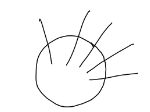
\includegraphics[width=0.5\linewidth]{normalenraum_kugel}
    \label{fig:normalenraum_kugel}
  \end{figure}
  \begin{eigenschaftenenumerate}
    \item \( \normalenraum{M}=\set{\lambda a|\lambda\in \reals} \).
    \item \( a\in \sphere{2} \), \( a_3>0 \).
    \begin{align*}
      \normalenraum{M}&=\Set{\varv|\varv_1=\frac{a_1}{\sqrt{1-a_1^2-a_2^2}}\varv_3,\varv_2=\frac{a_1}{\sqrt{1-a_1^2-a_2^2}}\varv_3}\\
      &=\Set{\lambda\frac{1}{\sqrt{1-a_1^2-a_2^2}}\begin{pNiceMatrix} a_1 \\ a_2 \\ \sqrt{\cdots} \end{pNiceMatrix}|\lambda\in\reals}=\Set{\lambda a|\lambda\in \reals}.
    \end{align*}
    \item Für allgemeinere Punkte als den Nordpol wäre dies mit Rechenaufwand verbunden.
  \end{eigenschaftenenumerate}
\end{beispiel*}
\approxtimestamp{25}
\begin{definition}\index{Stetig differenzierbare Abbildung von Untermannigfaltigkeiten}
  Sei \( M \) \( d \)-dimensionale Untermannigfaltigkeit des \( \reals^m \), sei \( N \) \( d' \)-dimensionale Untermannigfaltigkeit des \( \reals^n \). Eine Abbildung \( f\maps M\to N \) heißt \emph{stetig differenzierbar}, falls für alle \( a\in M \) gilt: Wenn \( \varphi\maps M\cap U \) eine lokale Parametrisierung bei \( a \) ist, so ist \( f\circ \varphi\maps\reals^d\supset V\to \reals^n \) stetig differenzierbar.
\end{definition}
\begin{bemerkungen*}
  Ist \( X\circ \varphi \) für eine lokale Parametrisierung \( \stetigefunktionen[1] \) und \( \psi\maps \tilde{V}\to M\cap \tilde{U} \) weitere Parametrisierung bei \( a \), so ist auch \( \evaluateat{X\circ \psi}{\inverse{\psi}(M\cap U\cap \tilde{U})} \) \( \stetigefunktionen[1] \), denn
  \begin{equation*}
    \evaluateat{X\circ \psi}{\inverse{\psi}(M\cap U\cap \tilde{U})}=\evaluateat{X\circ \varphi\circ \braceannotate{\text{Diffeo (\ref{tangentialraum_durch_parametisierung})}}{\inverse{\varphi}\circ\psi}}{\inverse{\psi}(M\cap U\cap \tilde{U})}.
  \end{equation*}
  \begin{figure}[H]
    \centering
    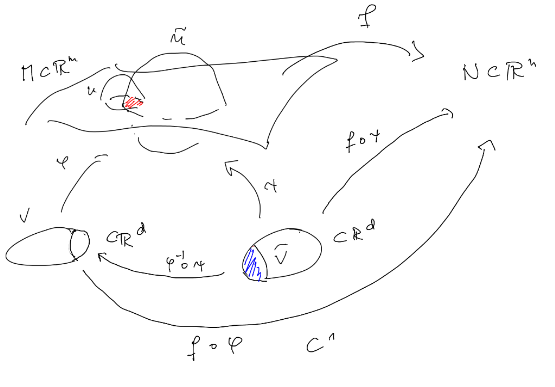
\includegraphics[width=1\linewidth]{uebertragung_stetige_diffbarkeit_auf_andere_parametisierung} % ChkTeX 25
    \caption*{\( \evaluateat{f\circ \psi}{
\includegraphics[height=\baselineskip]{uebertragung_stetige_diffbarkeit_auf_andere_parametisierung_blau}}=\evaluateat{f\circ \varphi\circ \braceannotate{\text{Diffeo}}{\inverse{\varphi}\circ \psi}}{
\includegraphics[height=\baselineskip]{uebertragung_stetige_diffbarkeit_auf_andere_parametisierung_blau}} \), \( 
\includegraphics[height=\baselineskip]{uebertragung_stetige_diffbarkeit_auf_andere_parametisierung_blau}= % ChkTeX 25
    \inverse{\psi}(\braceannotate{=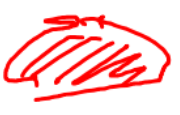
\includegraphics[height=\baselineskip]{uebertragung_stetige_diffbarkeit_auf_andere_parametisierung_rot}}{M\cap U\cap \tilde{U}}) \).} % ChkTeX 25
    \label{fig:uebertragung_stetige_diffbarkeit_auf_andere_parametisierung}
  \end{figure}
\end{bemerkungen*}
\begin{definition}\index{Vektorfeld}
  Sei \( M \) \( d \)-dimensionale Untermannigfaltigkeit des \( \reals^n \). Ein \emph{Vektorfeld} auf \( M \) ist eine stetig differenzierbare Abbildung 
  \begin{equation*}
    X\maps M\to \reals^n \logicspace \text{\sd}\logicspace  X(a)\in \tangentialraum{M}\quad \forall a\in M.
  \end{equation*}. Ein \emph{Normalenfeld} ist eine stetig differenzierbare Abbildung 
  \begin{equation*}
    \mathcal{N}\maps M\to \reals^n \logicspace \text{\sd}\logicspace  \mathcal{N}(a)\in \normalenraum{M}\quad \forall a\in M.
  \end{equation*}
\end{definition}
\begin{beispiele*}
  \begin{enumerate}
  \item \( M=\sphere{5} \), \( \mathcal{N}(a)=a \) offensichtlich stetig differenzierbar.
  \item \( M= \) Torus \( \Pi^2\subset \reals^3 \), \( r<R \).
  \begin{equation*}
    f(x,y,z)=(x^2+y^2+z^2+R^2-r^2)^2-4R^2(x^2+y^2).
  \end{equation*}
  \( f=0 \) definiert eine Untermannigfaltigkeit:
  \begin{figure}[H]
    \centering
    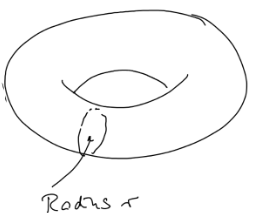
\includegraphics[width=0.5\linewidth]{torus}
    \label{fig:torus}
  \end{figure}
  \begin{equation*}
    \grad{f}(a)=\begin{pNiceMatrix} 4a_1(a_1^2+a_2^2+a_3^2-R^2-r^2) \\ 4a_2(a_1^2+a_2^2+a_3^2-R^2-r^2) \\ 4a_3(a_1^2+a_2^2+a_3^2+R^2-r^2) \end{pNiceMatrix}\neq 0
  \end{equation*}
  für \( a\in  \Pi^2 \) \timplies \( Df(a) \) hat maximalen Rang (\( 1 \)).
  \begin{equation*}
    \mathcal{N}(a)=\frac{\grad{f(a)}}{\euclidiannorm{\grad{f(a)}}}
  \end{equation*}
  ist stetig differenzierbar.
  \emph{Tangentialraum} \( \tangentialraum{M}= \) Ebene senkrecht \( \varv_a=\grad{f(a)} \). Parametrisierung bei \( a\in \Pi^2 \): Mit geeigneten Intervallen für die Winkel gilt:
  \begin{gather*}
    a=\varphi(\alpha,\beta)=R\begin{pNiceMatrix} \Cos{\alpha} \\ \Sin{\alpha} \\ 0 \end{pNiceMatrix}+r\begin{pNiceMatrix} \Cos{\alpha}\Cos{\alpha} \\ \Sin{\alpha}\Cos{\beta} \\ \Sin{\beta} \end{pNiceMatrix}\\
    X(\phi(\alpha,\beta))=\partial_2 \varphi(\alpha,\beta)=\begin{pNiceMatrix} -r\Cos{\alpha}\Sin{\beta} \\ -r\Sin{\alpha}\Sin{\beta} \\ \Cos{\beta} \end{pNiceMatrix}
  \end{gather*}
  offensichtlich \( \stetigefunktionen[1] \).
  \begin{figure}[H]
    \centering
    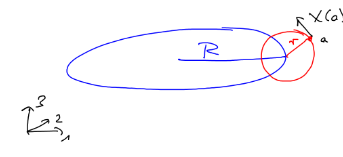
\includegraphics[width=0.5\linewidth]{parametisierung_torus_durch_winkel}
    \label{fig:parametisierung_torus_durch_winkel}
  \end{figure}
  \begin{figure}[H]
    \centering
    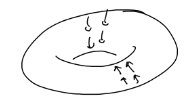
\includegraphics[width=0.5\linewidth]{vektorfeld_auf_torus}
    \label{fig:vektorfeld_auf_torus}
  \end{figure}
  \item Möbius-Band. 
  \begin{figure}[H]
    \centering
    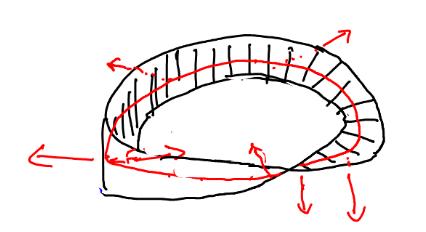
\includegraphics[width=0.5\linewidth]{moebius_band}
    \label{fig:moebius_band}
  \end{figure}
  Langer Streifen Papier, einmal verdrehen, zusammenkleben. Mittellinie einzeichnen. Normalenvektor auf einem Punkt der Mittellinie bestimmen, auf \( 1 \) normieren (\( \euclidiannorm{\varv}=1 \)). Führt man diesen stetig entlang der Mittellinie und verändert dabei seine Länge nicht, sieht man, dass es kein stetiges normiertes Normalenfeld auf dem Möbius-Band geben kann. Eine solche Fläche nennt man nicht orientierbar. 
  \end{enumerate}
\end{beispiele*}
\begin{definition}\index{Integralkurve}
  Sei \( X\maps M\to \reals^n  \) ein Vektorfeld (\( M \) \( d \)-dimensionale Untermannigfaltigkeit). Eine \emph{Integralkurve} von \( X \) ist eine stetig differenzierbare Kurve \( \gamma\maps I\to M \) \sd
  \begin{equation*}
    \gamma'(t)=X(\gamma(t))
  \end{equation*}
  Im nächsten Kapitel (Differenzialgleichungen) wird es um Existenz und Eindeutigkeit solcher Kurven gehen (aber nur im \( \reals^n \)).
\end{definition}
\begin{definition}\index{Untermannigfaltigkeit mit Rand}\label{untermannigfaltigkeit_mit_rand}
  \( M\subset \reals^n \) ist eine \( d \)-dimensionale \emph{Untermannigfaltigkeit mit Rand} falls es zu jedem \( a\in M \) eine lokale Parametrisierung gibt \( \varphi\maps V\to \varphi(V)\subset M \) mit \( V\subset \reals^d_{-} \), \( \reals^d_{-}=\Set{x\in \reals^d|x_1\leq 0} \) (\( V \) offen in \( \reals^d_{-} \), falls \texists  \( U \) offen in \( \reals^d \) \sd \( V=\reals^d_{-}\cap U \) (Teilraumtopologie), also \zb ist \( \ointerval{\infty}{0}\times \ointerval{0}{1}^{d-1} \) offen in \( \reals^{d}_{-} \)). \( p \) heißt \emph{Randpunkt von \( M \)}, falls \( p=\varphi(t) \) mit \( t\in V\cap \partial \reals^d_{-} \), wobei
  \begin{equation*}
    \partial \reals^d_{-}=\Set{(0,x_2,\dotsc,x_{d})\in \reals^d_{-}}.
  \end{equation*}
  Die Menge aller Randpunkte wird mit \( \partial M \) bezeichnet.
\end{definition}
\begin{bemerkung*}
  Man kann auch \( \reals_{+}^d=\Set{x\in \reals^d|x_1\geq 0} \) oder auch \( \Set{x\in \reals^d|x_d\geq c} \) \bzw \( \Set{x\in \reals^d|x_d\leq c} \) betrachten.
\end{bemerkung*}
\begin{beispiel*}
  \( \overline{\mathbb{D}}=\Set{x\in \reals^2| \euclidiannorm{x}\leq 1} \). \( \overline{\partial \mathbb{D}}=\sphere{1} \). Wähle zu \( a\in \overline{\mathbb{D}} \), \( a\neq \transpose-{(1,0)} \). Sei \( V=\rinterval{0}{1}\times \ointerval{0}{2\pi} \). Dann ist \( V \) offen in \( \Set{x\in \reals^2|x_1\leq 1} \) und \( V\cap \Set{x|x_1=1}=\sphere{1}\setminus \Set{(1,0)} \).
  \begin{equation*}
    \varphi\maps \braceannotate{=V}{\rinterval{0}{1}\times \ointerval{0}{2\pi}}\to \reals^2\quad \varphi(r,\alpha)=r\transpose-{(\Cos{\alpha},\Sin{\alpha})}.
  \end{equation*}
  Analog zu \( a=\transpose-{(1,0)} \).
  \begin{gather*}
    \varphi\maps \rinterval{0}{1}\times \ointerval{-\pi}{\pi}\to \reals^2\quad \varphi(r,a)=r\transpose-{(\Cos{\alpha},\Sin{\alpha})}.
  \end{gather*}
\end{beispiel*}
\timestamp{Ende Audio Teil 1}
\section{Flächenbemessung auf Untermannigfaltigkeiten}
\begin{definition*}\index{Erste Fundamentalform}
  \begin{gather*}
    I_a\definedas \scalarproduct{\cdot}{\cdot}_a\maps \tangentialraum{M}\times\tangentialraum{M}\to \reals\\
    I_a(v,w)=\scalarproduct{v}{w}_{a}=\scalarproduct{v}{w}_{\text{E}}\quad \forall v,w\in \tangentialraum{M}
  \end{gather*}
  heißt \emph{erste Fundamentalnorm}.
\end{definition*}
\begin{bemerkung*}
  \( \tangentialraum{M}=\Span-{\Set{\partial_1 \varphi(t_0),\dotsc,\partial_d \varphi(t_0)}} \), \( \varphi\maps V\to M\cap U \) Parametrisierung bei \( a \), \( \varphi(t_0)=a \). Es gilt für \( v=\sum v_i \partial_i \varphi(t_0) \), \( w=\sum w_i \partial_i \varphi(t_0) \)
  \begin{align*}
    \scalarproduct{v}{w}_{a}&=\scalarproduct*{\sum v_i \partial_i \varphi(t_0)}{w_j \partial_j \varphi(t_0)}_{a}\\
    &=\sum_{i}\sum_j v_i w_j \braceannotate{\defines g_{ij}(t_0)}{\scalarproduct{\partial_i \varphi(t_0)}{\partial_j \varphi(t_0)}_{\text{E}}}.
  \end{align*}
  \( g\definedas \parens{g_{ij}}_{\substack{i=1,\dotsc,d\\ j=1,\dotsc,d}}\maps V\to \reals \) heißt \emph{metrischer Tensor} (oder Gramsche Matrix).
\end{bemerkung*}
\begin{lemma}\label{parameterwechsel_metrischer_tensor}
   Unter Parameterwechsel (\vgl \ref{parameterwechsel}) verhält sich der metrischer Tensor wie folgt:
   \begin{equation*}
     \explain{\text{bezgl.\ \( \psi\maps \tilde{V}\to M\cap \tilde{U} \) berechnet}}=\transpose{D\Phi(s)}\explain[big]{\text{bezgl.\ \( \varphi\maps V\to M\cap U \) berechnet}}{g_{\varphi}}(\Phi(s))D\Phi(s)
   \end{equation*}
   mit
   \begin{equation*}
    \Phi=\inverse{\varphi}\circ \psi\maps  \inverse{\varphi}(M\cap U\cap \tilde{U})\to \inverse{\varphi}(M\cap U\cap \tilde{U}).
   \end{equation*}
\end{lemma}
\begin{proof}
  Betrachte \( \psi=\varphi\circ \Phi \). Kettenregel liefert
  \begin{equation*}
    \scalarproduct{\partial_k \psi}{\partial_l \psi}=\sum_{i,j}\scalarproduct{\partial_i \varphi}{\partial_j \varphi}\partial_k \Phi_i\partial_l \Phi_j.
  \end{equation*}
\end{proof}
\begin{frage}
  Was hat \( g \) mit Flächenmessung zu tun?
  \begin{eigenschaftenenumerate}
    \item Wir betrachten eine Hyperfläche
     (\( M=(n-1) \)-dimensional,
      also hier \( d=2 \)) 
      \( M\subset \reals^3\).
       Sei \( M\cap U\subset \reals^3 \) parametrisiert von 
       \( \varphi\maps V\to M\cap U \). Dann ist
    \begin{equation*}
      \varphi(t_0+h)=\varphi(t_0)+D\varphi(t_0)\matrixmult h+R_{t_0}(h).
    \end{equation*}
    Wir wollen dies nutzen, um die Fläche von \( A \) abzuschätzen.
    \begin{figure}[H]
      \centering
      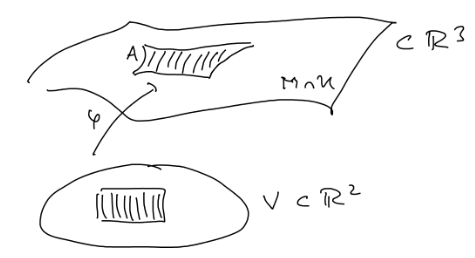
\includegraphics[width=0.5\linewidth]{flaeche_auf_mannigfaltigkeit}
      \label{fig:flaeche_auf_mannigfaltigkeit}
    \end{figure}
    \item Zunächst: Sei \( \mathcal{R}=\interval{a_0}{a_0+l_1}\times \interval{b_0}{b_0+l_2}\subset V \). Dann ist, wenn man die Restterme vernachlässigt \( \varphi(\mathcal{R}) \) ungefähr (\( t_0=\transpose-{(a_0,b_0)} \))
    \begin{equation*}
      \varphi(t_0)+D\varphi(t_0)\matrixmult \begin{pNiceMatrix} a_0 \\ b_0 \end{pNiceMatrix}+P(l_1 \partial_1 \varphi(t_0),l_2 \partial_2 \varphi(t_0)),
    \end{equation*}
    wobei \( P(v,w) \) das Parallelotop ist, dass von \( v,w\in \reals^3 \) aufgespannt wird,
    \begin{equation*}
      P(v,w)=\Set{s_1 v+s_2 w|0\leq s_j\leq 1}.
    \end{equation*}
    Denn für \( h\in \reals^2 \) gilt
    \begin{equation*}
      D\varphi(t_0)\matrixmult h=h_1 \partial_1 \varphi(t_0)+h_2 \partial_2 \varphi(t_0)\in \reals^3
    \end{equation*}
    und allgemein gilt für \( v ,w \in \reals^3\) und
    \begin{gather*}
      r_{v,w}=r\maps \mathcal{R}\to \reals^3\quad r\begin{pNiceMatrix} h_1 \\ h_2 \end{pNiceMatrix}=h_1 v+ h_2 w\\
      r(\mathcal{R})=\braceannotate{=p}{r(t_0)}+P(l_1 v, l_2 w).
    \end{gather*}
    \begin{figure}[H]
      \centering
      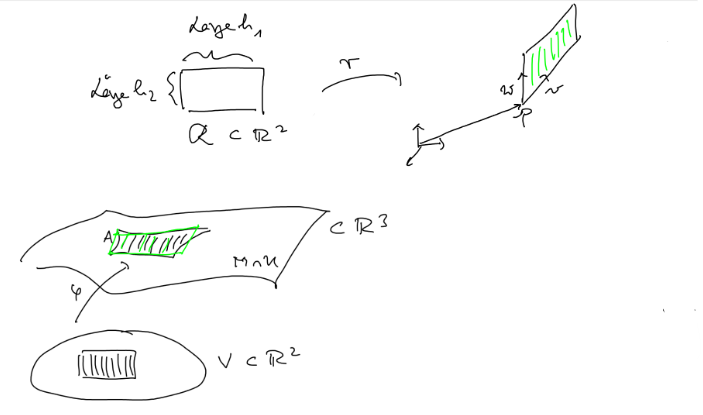
\includegraphics[width=1\linewidth]{flaechenmessung_mit_parallelotopen}
      \label{fig:flaechenmessung_mit_parallelotopen}
    \end{figure}
    Zur ungefähren Berechnung des Flächeninhaltes von \( \varphi(\mathcal{R}) \) berechnen wir also den des Parallelotops \( P(\partial_1 \varphi(t_0)l_1,\partial_2 \varphi(t_0)l_2) \).
    \item Seien \( v,w\in \reals^3 \). Dann ist \( \norm{v\times w} \), \( v\times w=\begin{pNiceMatrix} v_2 w_3-v_3w_2 \\ v_3 w_1 -v_1 w_3 \\ v_1 w_2-v_2 w_1 \end{pNiceMatrix} \), \enquote{\emph{Kreuzprodukt}} der Flächeninhalt des Parallelotops \( P(v,w) \). Den:
    \begin{align*}
      A&=\norm{v}\cdot\norm{w}\cdot\Sin{\beta}\\
      &=\sqrt{\norm{v}^2\norm{w}^2(1-\Cos+{\beta}^2)}\\
      &=\sqrt{\norm{c}^2\norm{w}^2-\scalarproduct{v}{w}^2}\\
      &=\sqrt{\norm{v\times w}^2}=\norm{v\times w}
    \end{align*}
    mit \( \times \) wie oben.
    \item Es gilt
    \begin{equation*}
      \label{eq:flaecheninhalt_durch_determinante_gegeben}\tag{*} \euclidiannorm{\partial_1 \varphi(t_0)\times\partial_2 \varphi(t_0)}=\sqrt{\determinant{g_{\varphi}(t_0)}}
    \end{equation*}
    mit \( \determinant{g_{\varphi}}= \) Determinante der Gramschen Matrix. Also ist die Fläche von \( \varphi(R) \) etwa 
    \begin{equation*}
      \sqrt{g_{\varphi}(t_0)}l_1 l_2=\sqrt{g_{\varphi}(t_0)}\text{Fläche}(\mathcal{R}).
    \end{equation*}
    Die Determinante gibt also an, wie sehr doe Fläche von \( \mathcal{R} \) gestaucht oder gestreckt wird.

    Wir werden uns später überlegen, wie man ausgehend von den hier skizzierten Ideen zu einer Definition des Flächeninhalts kommt, der nicht von der gewählten Parametrisierung abhängt.
  \end{eigenschaftenenumerate}
  Es ist noch \eqref{eq:flaecheninhalt_durch_determinante_gegeben} zu zeigen.
  \begin{lemma}\label{berechnung_gramsche_determinante}
    Sei \( \varphi\maps V\to M\cap U \) Parametrisierung bei \( a \), \( V\subset \reals^d \), \( M\subset \reals^n \). Die Determinante von \( g_{ij} \) berechnet sich wie folgt:
    \begin{equation*}
      \determinant{g(t_0)}=\sum_{i_1<\dotsb<i_d}\parens*{\determinant{D\begin{pNiceMatrix} \varphi_{i_1} \\ \Vdots \\ \varphi_{i_j} \end{pNiceMatrix}(t_0)}}^2
    \end{equation*}
  \end{lemma}
  \begin{proof}
    \begin{equation*}
      g(t_0)=\transpose{(D\varphi)(t_0)}\matrixmult D\varphi(t_0)
    \end{equation*}
    und lineare Algebra (Satz von Cauchy-Binet)
    
  \end{proof}
\end{frage}
\begin{bemerkung*}
  Für \( d=2 \), \( n=3 \) gilt nun
  \begin{align*}
    \determinant{g_{\varphi}}&=\sum_{i<j}\p*{ \determinant{D\begin{pNiceMatrix} \phi_i \\ \phi_j \end{pNiceMatrix} }}^2\\
    &=\determinant{D\begin{pNiceMatrix} \varphi_1 \\ \varphi_2 \end{pNiceMatrix}}^2+\determinant{D\begin{pNiceMatrix} \varphi_1 \\ \varphi_3 \end{pNiceMatrix}}^2+\determinant{D\begin{pNiceMatrix} \varphi_2 \\ \varphi_3 \end{pNiceMatrix}}^2\\
    &\explain{\text{Rechnung}}{=}\scalarproduct{\partial_1 \varphi \times \partial_2 \varphi}{\partial_1 \varphi\times \partial_2 \varphi}\implies \text{\Beh \eqref{eq:flaecheninhalt_durch_determinante_gegeben}}.
  \end{align*}
\end{bemerkung*}